\documentclass[tikz,border=6pt]{standalone}
\usepackage{pgfplots}
\pgfplotsset{compat=1.18}
\begin{document}
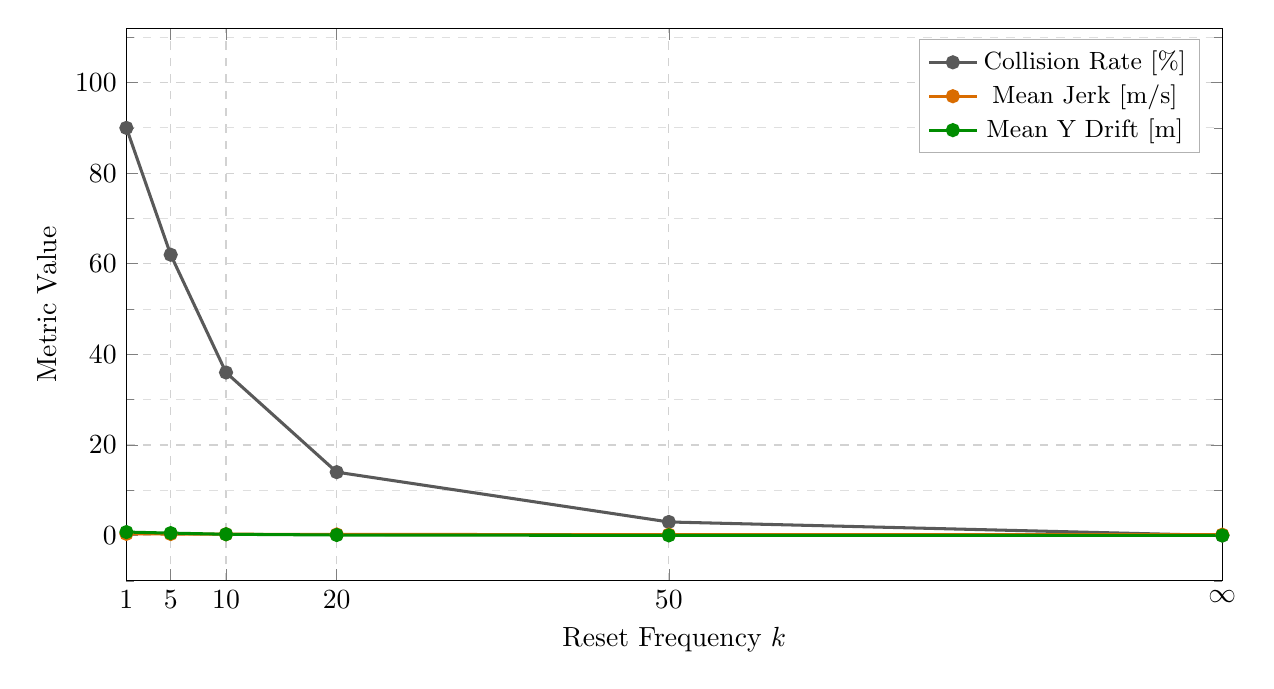
\begin{tikzpicture}
\begin{axis}[
width=15.5cm,
height=8.6cm,
xmin=1, xmax=100,
ymin=-10, ymax=112,
grid=both,
grid style={draw=gray!25,dashed},
major grid style={draw=gray!35,dashed},
minor tick num=1,
axis background/.style={fill=white},
legend style={at={(0.98,0.98)},anchor=north east,legend columns=1,fill=white,draw=black!30,font=\small},
xlabel={Reset Frequency $k$},
ylabel={Metric Value},
xtick={1,5,10,20,50,100},
xticklabels={$1$,$5$,$10$,$20$,$50$,$\infty$},
]
\addplot+[thick,mark=*,color=gray!70!black,line width=1.1pt,mark options={fill=gray!70!black}] coordinates {(1,90.0) (5,62.0) (10,36.0) (20,14.0) (50,3.0) (100,0.0)};
\addlegendentry{Collision Rate [\%]}
\addplot+[thick,mark=*,color=orange!85!black,line width=1.1pt,mark options={fill=orange!85!black}] coordinates {(1,0.376) (5,0.342) (10,0.298) (20,0.244) (50,0.209) (100,0.198)};
\addlegendentry{Mean Jerk [m/s]}
\addplot+[thick,mark=*,color=green!55!black,line width=1.1pt,mark options={fill=green!55!black}] coordinates {(1,0.770) (5,0.542) (10,0.286) (20,0.118) (50,0.041) (100,0.022)};
\addlegendentry{Mean Y Drift [m]}
\end{axis}
\end{tikzpicture}
\end{document}
